\documentclass[conference]{IEEEtran}

% Packages
\usepackage[utf8]{inputenc}
\usepackage[english]{babel}
\usepackage{amsmath}
\usepackage{amsfonts}
\usepackage{amssymb}
\usepackage{amsthm}
\usepackage{pdfpages}
\usepackage{graphicx}
\usepackage{epstopdf}
\usepackage{listings}
\usepackage{cite}
\usepackage{enumerate}
\usepackage{scientific}
\usepackage[colorlinks=false]{hyperref}
\usepackage{bookmark}

\usepackage[]{mcode}	%Matlab Code
\usepackage{tikz,pgfplots}	%Tikz

%\usepgfplotslibrary{external} 
%\tikzexternalize
%\tikzsetexternalprefix{ext/}

% Bookmark Setup
\bookmarksetup{numbered}

% PDF Setup
\hypersetup{pdftitle={Homework 7}, pdfsubject={Documentation of 7th Homework}, pdfauthor={Stefan Röhrl}, pdfkeywords={Neuroprothetik Exercise}, pdfcreator={LaTeX}, hidelinks}


\begin{document}
%
% cite all references
%\nocite{*}
%
% paper title
% can use linebreaks \\ within to get better formatting as desired
\title{Homework 7\\ CI Signalverarbeitung}

\author{\IEEEauthorblockN{Stefan Röhrl}
\IEEEauthorblockA{Technische Universität München, Arcisstraße 21, Munich, Germany\\
Email: stefan.roehrl@tum.de}}

% use for special paper notices
%\IEEEspecialpapernotice{(Invited Paper)}

% make the title area
\maketitle

\IEEEpeerreviewmaketitle

\section{Frequenzgang}

\begin{figure}[h]
	\centering
	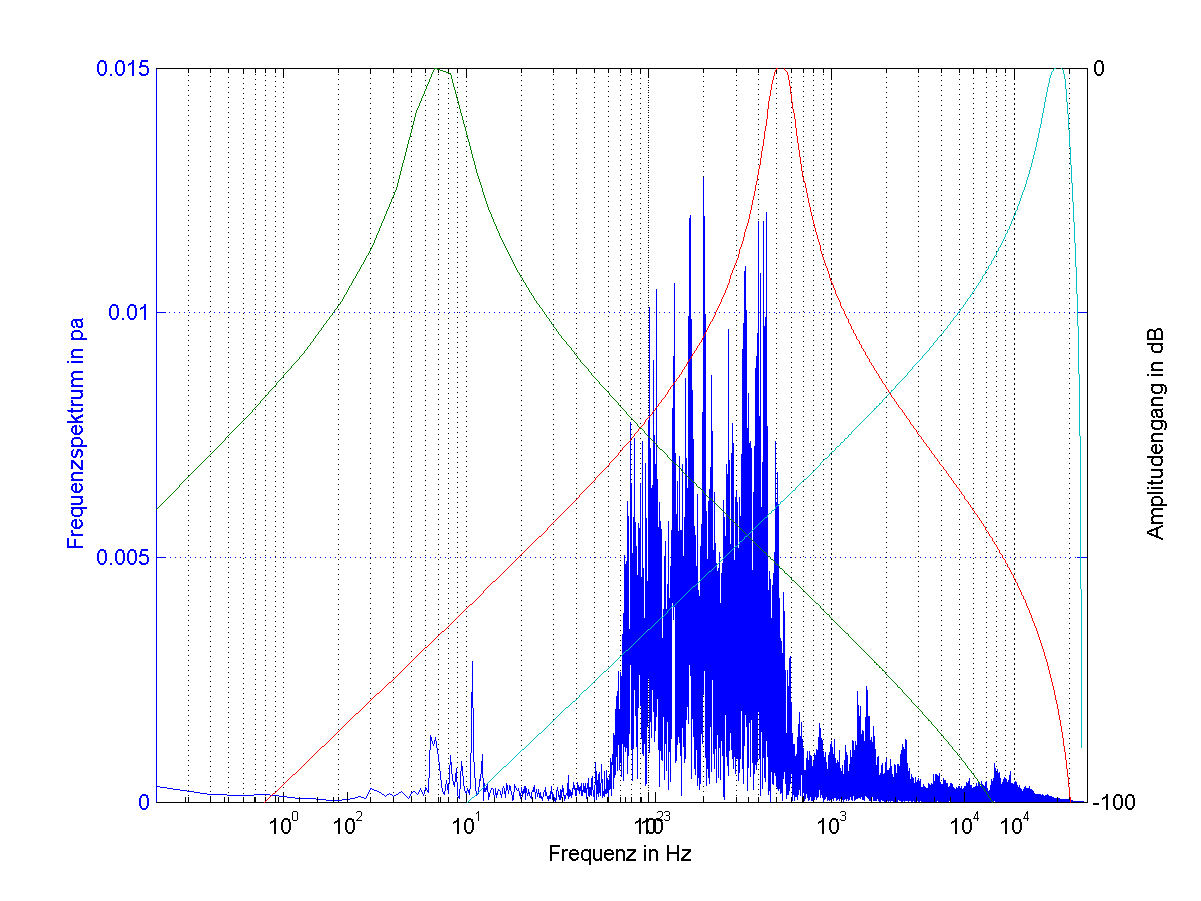
\includegraphics[width=0.5\textwidth]{img/freq_gang_3.png}
	\caption{Frequenzgang für 3 Kanäle}
	\label{fig:freq-gang-3}
\end{figure}

\begin{figure}[h]
	\centering
	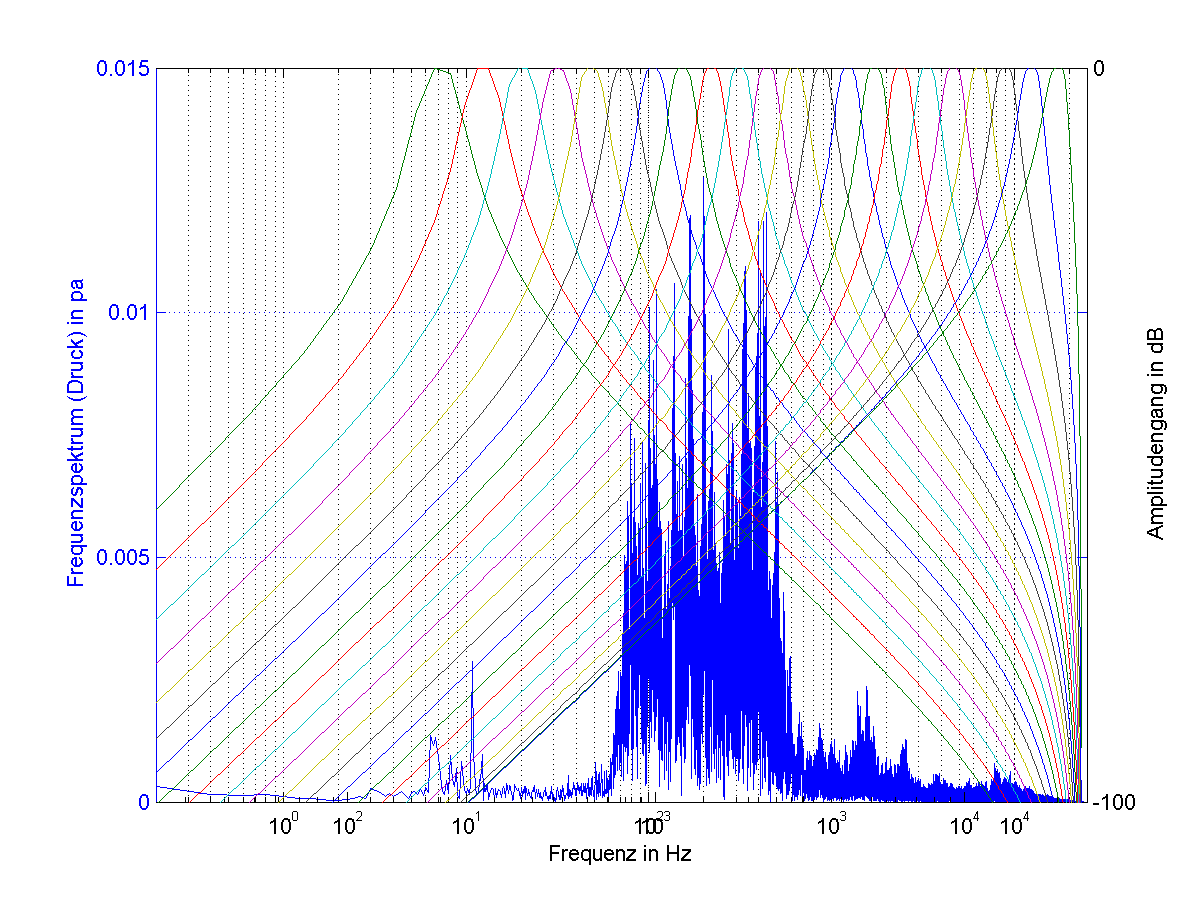
\includegraphics[width=0.5\textwidth]{img/freq_gang_22.png}
	\caption{Frequenzgang für 22 Kanäle}
	\label{fig:freq-gang-22}
\end{figure}

\section{Filterbank}

\begin{figure}[h]
	\centering
	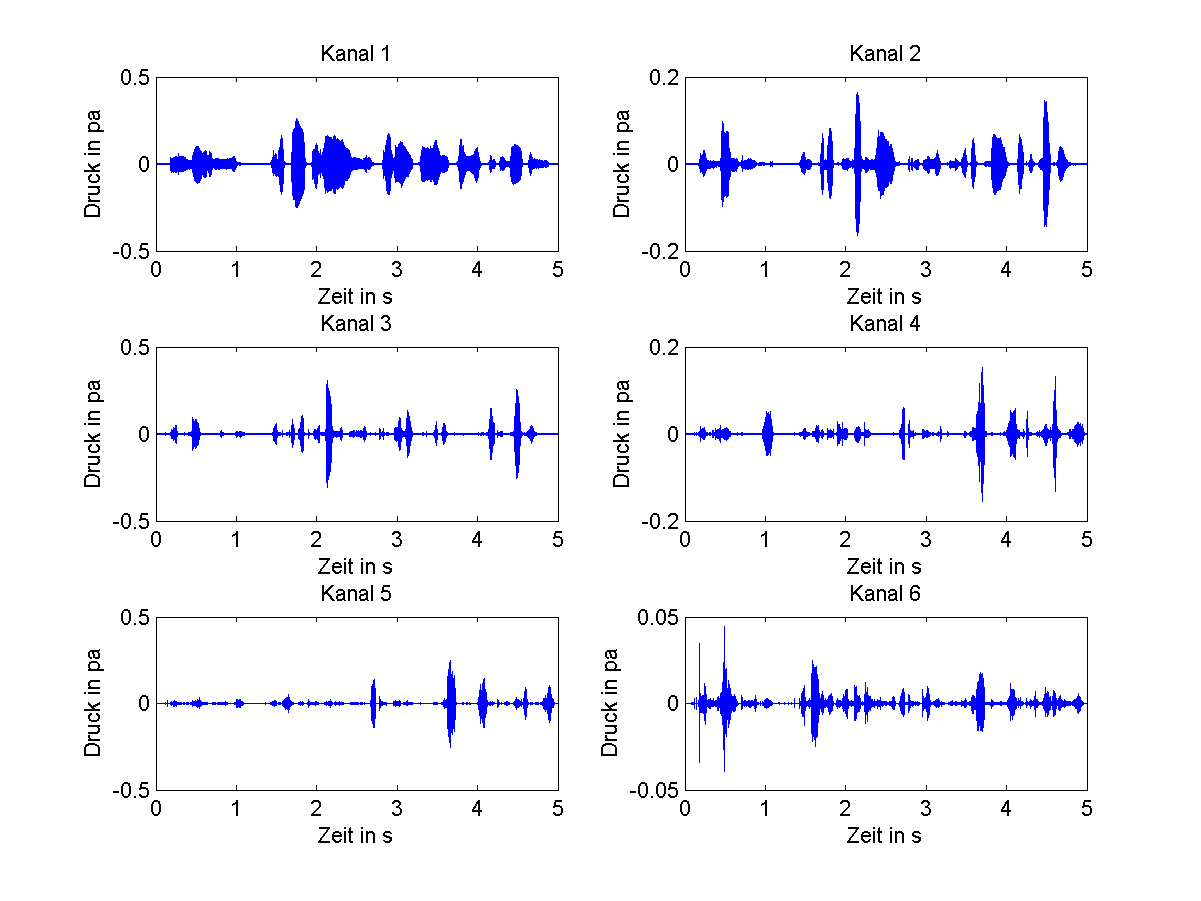
\includegraphics[width=0.5\textwidth]{img/fb_6.png}
	\caption{Gefilterte Signale mit 6 Kanälen}
	\label{fig:fb-6}
\end{figure}

\begin{figure}[h]
	\centering
	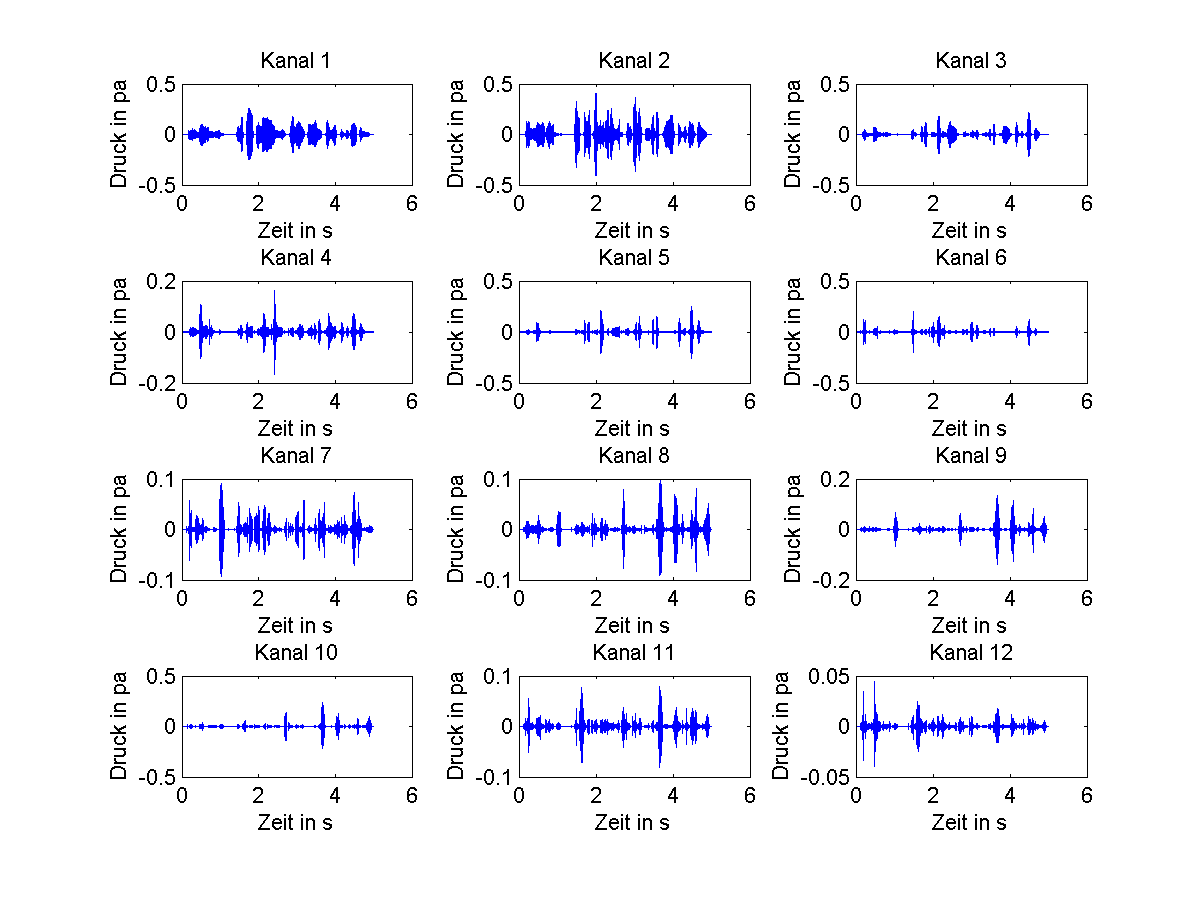
\includegraphics[width=0.5\textwidth]{img/fb_12.png}
	\caption{Gefilterte Signale mit 12 Kanälen}
	\label{fig:fb-12}
\end{figure}

\section{Kurzzeitspektrum}

\begin{figure}[h]
	\centering
	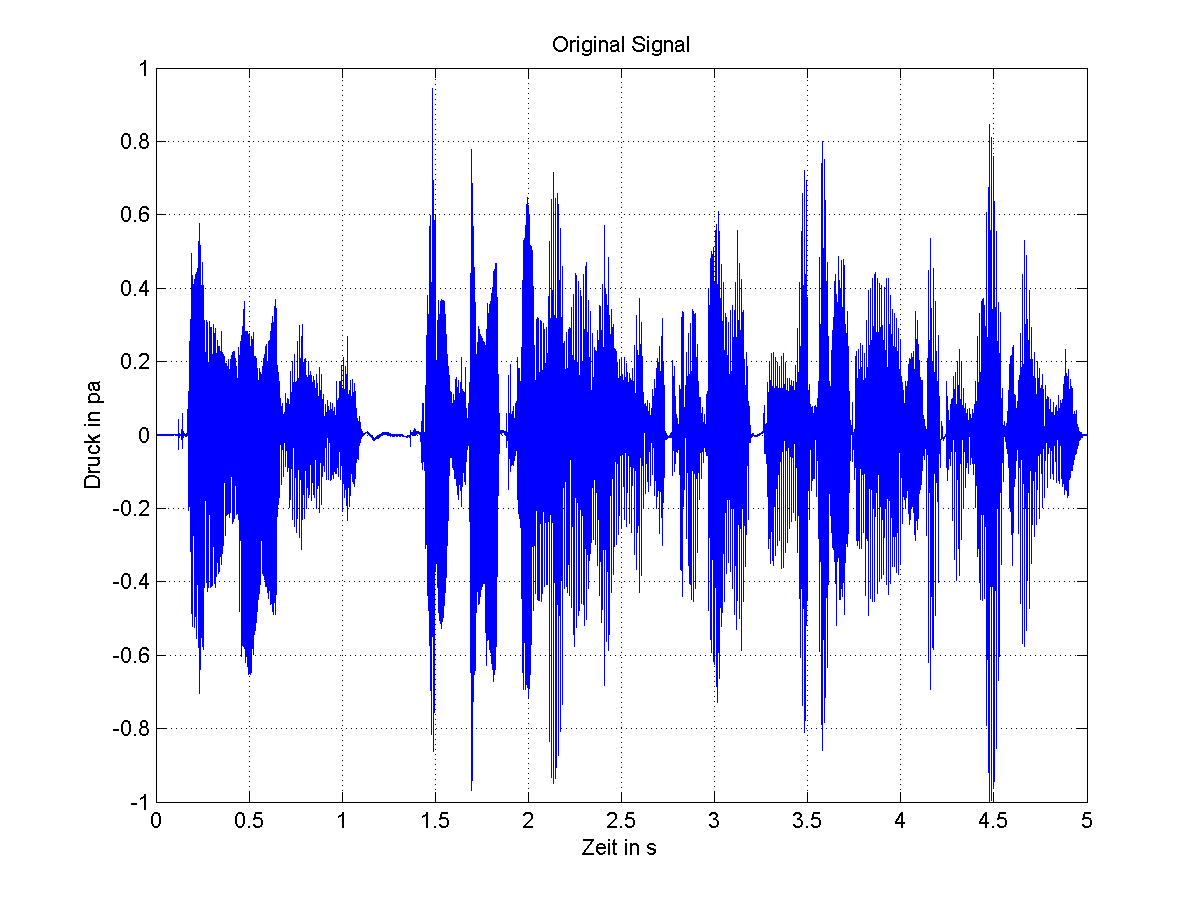
\includegraphics[width=0.5\textwidth]{img/sig_orig.png}
	\caption{Original Signal}
	\label{fig:sig-orig}
\end{figure}

\begin{figure}[h]
	\centering
	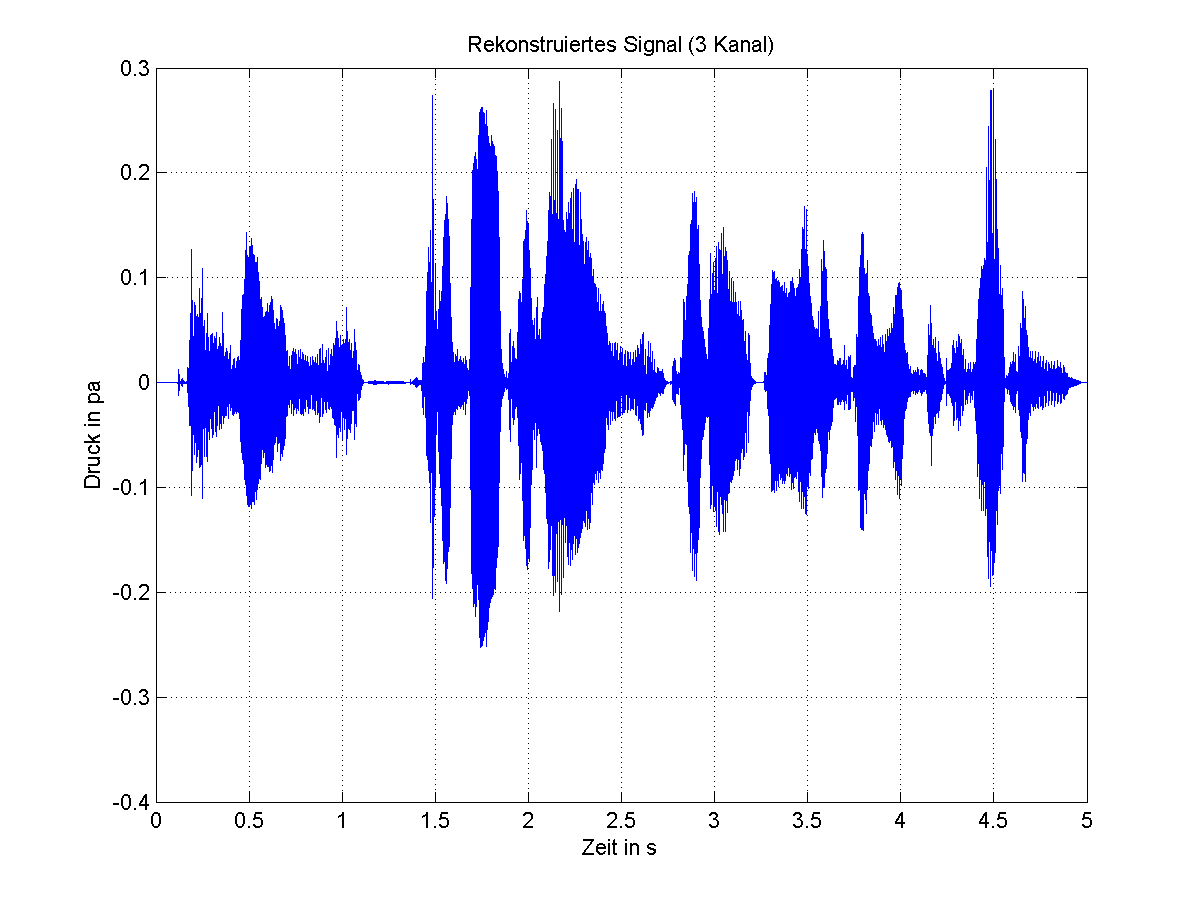
\includegraphics[width=0.5\textwidth]{img/sig_rec_3.png}
	\caption{Rekonstruiertes Signal von 3 Kanälen}
	\label{fig:sig-rec-3}
\end{figure}

\begin{figure}[h]
	\centering
	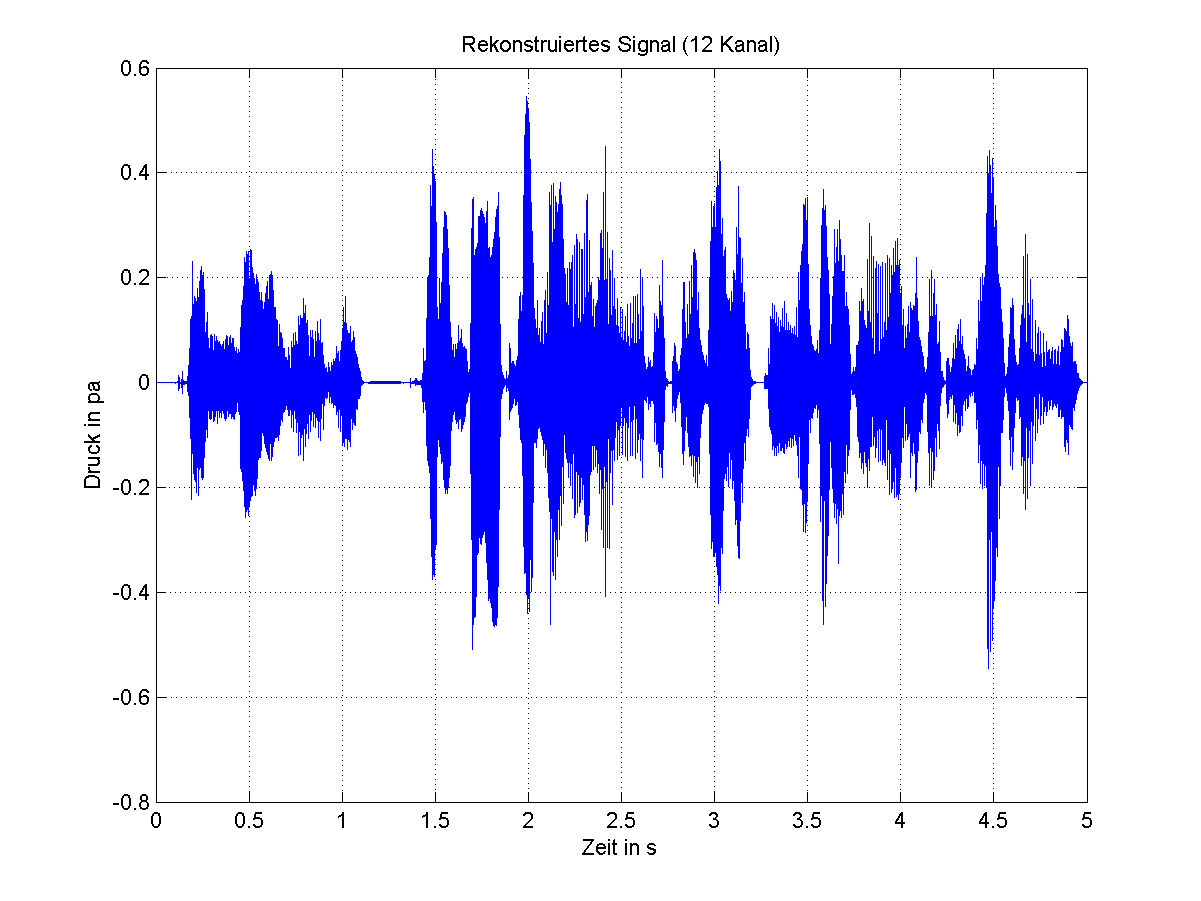
\includegraphics[width=0.5\textwidth]{img/sig_rec_12.png}
	\caption{Rekonstruiertes Signal von 12 Kanälen}
	\label{fig:sig-rec-12}
\end{figure}

\begin{figure}[h]
	\centering
	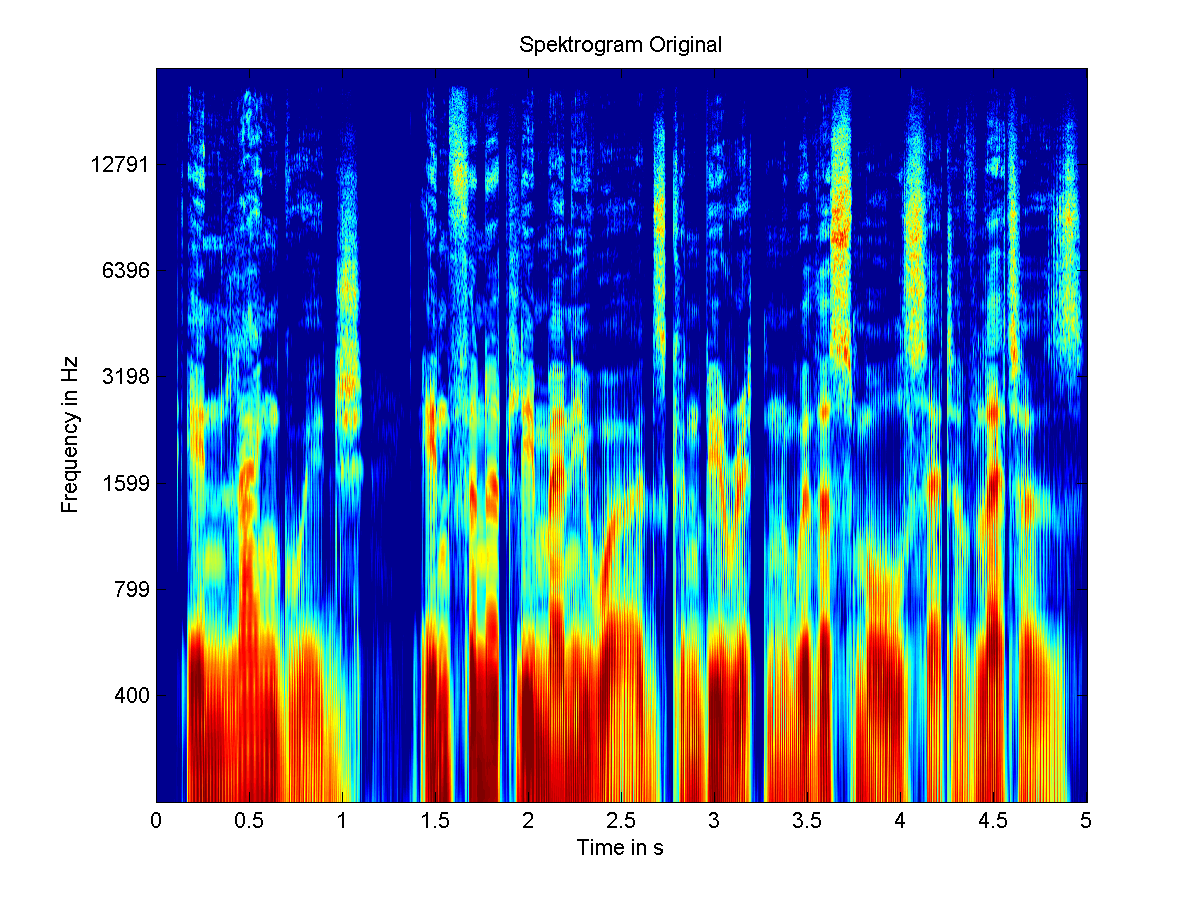
\includegraphics[width=0.5\textwidth]{img/spect_orig.png}
	\caption{Kurzzeitspektrum Original}
	\label{fig:spect-orig}
\end{figure}

\begin{figure}[h]
	\centering
	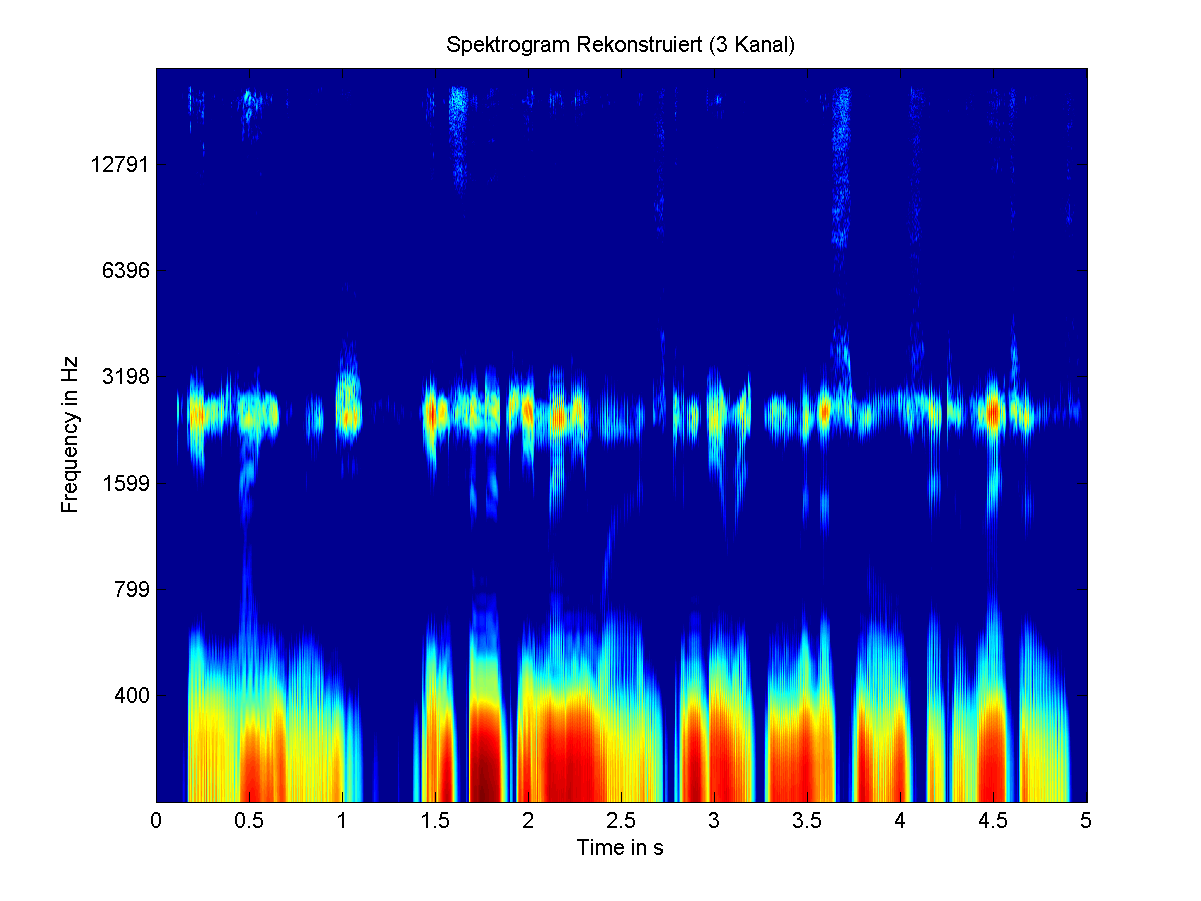
\includegraphics[width=0.5\textwidth]{img/spect_rec_3.png}
	\caption{Kurzzeitspektrum rekonstruiert von 3 Kanälen}
	\label{fig:spect-rec-3}
\end{figure}

\begin{figure}[h]
	\centering
	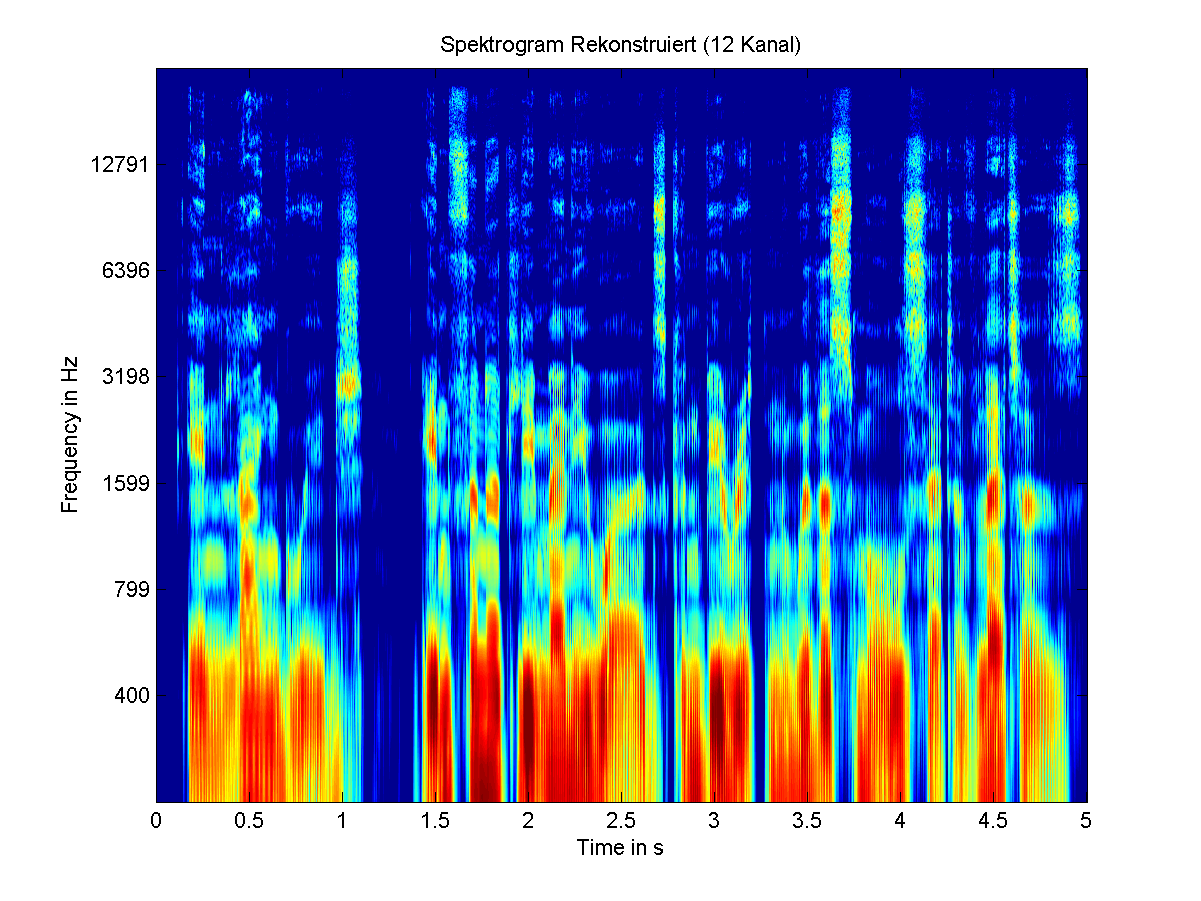
\includegraphics[width=0.5\textwidth]{img/spect_rec_12.png}
	\caption{Kurzzeitspektrum rekonstruiert von 12 Kanälen}
	\label{fig:spect-rec-12}
\end{figure}

\begin{figure}[h]
	\centering
	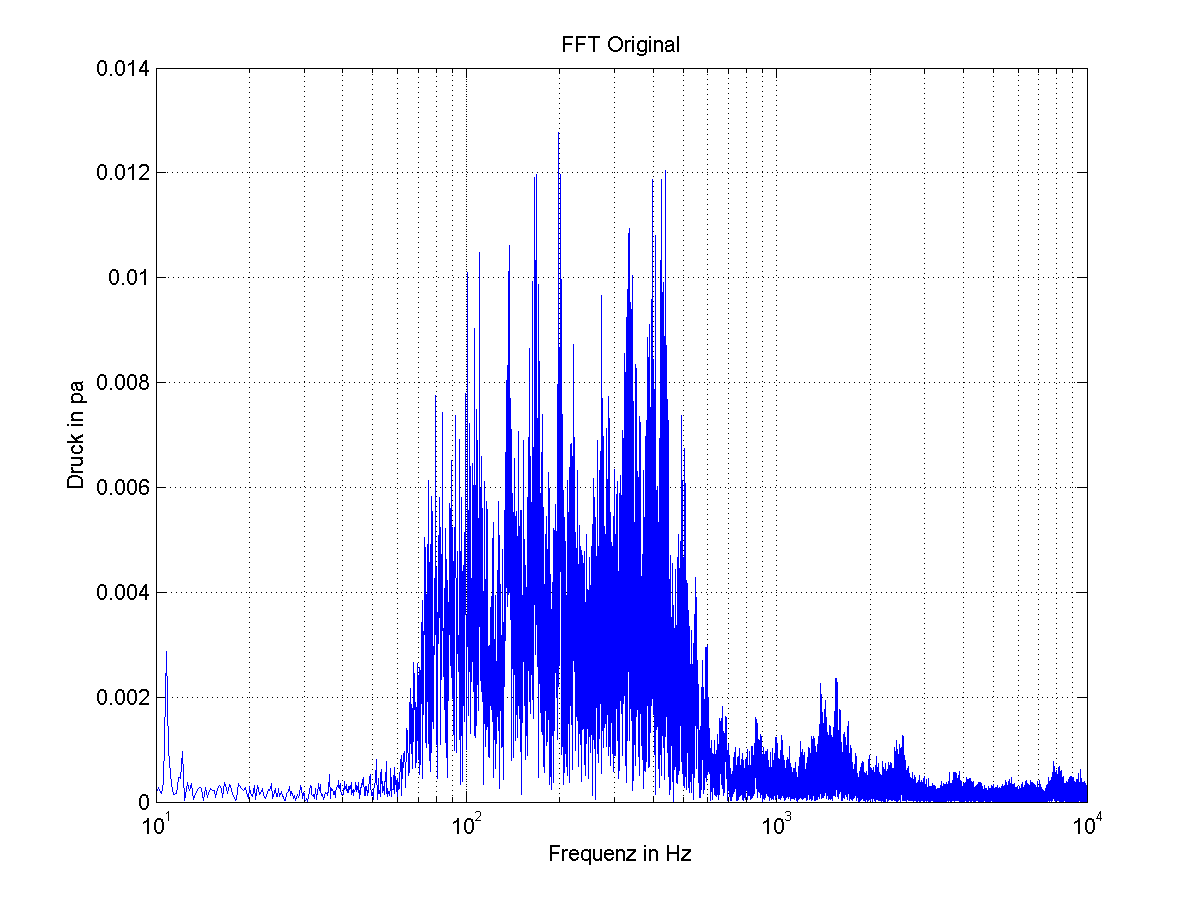
\includegraphics[width=0.5\textwidth]{img/fft_orig.png}
	\caption{Langzeitspektrum Original}
	\label{fig:fft-orig}
\end{figure}

\begin{figure}[h]
	\centering
	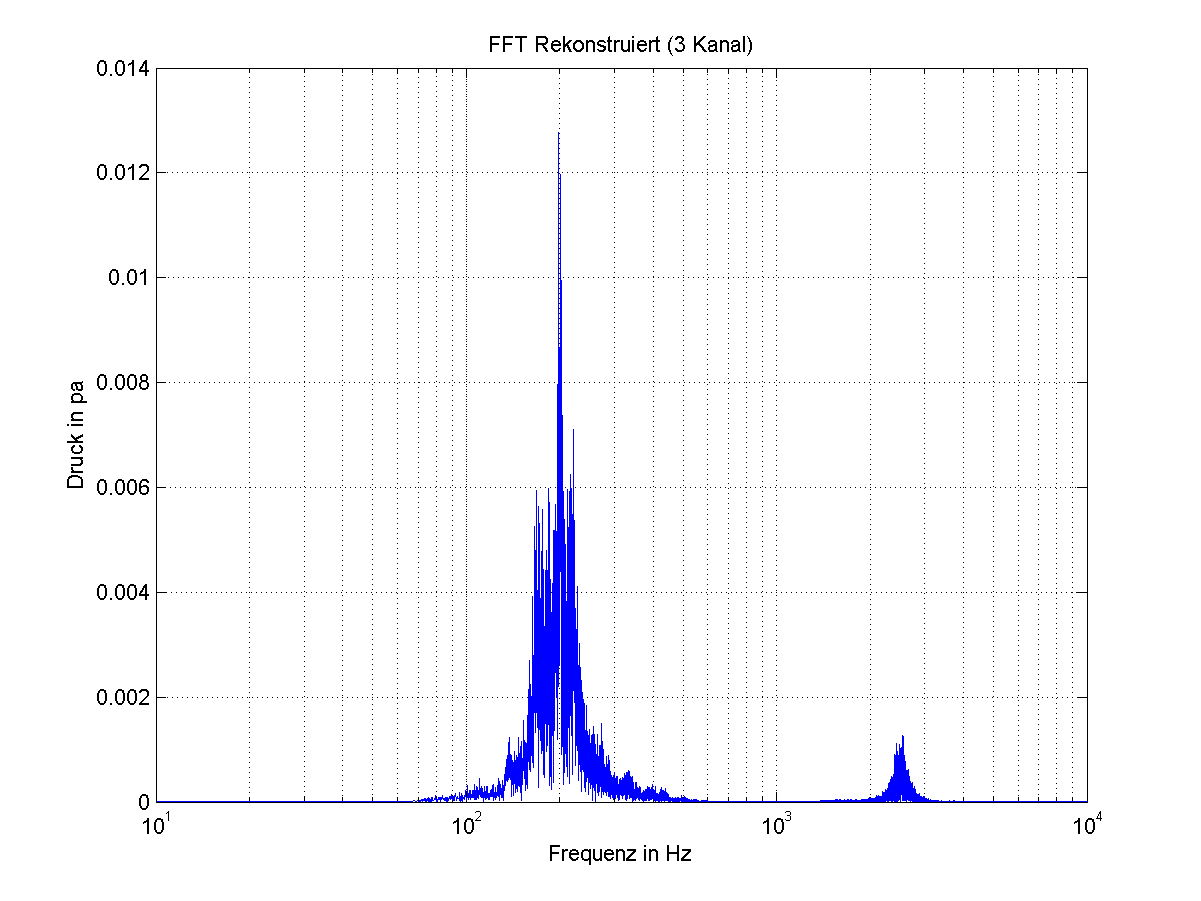
\includegraphics[width=0.5\textwidth]{img/fft_rec_3.png}
	\caption{Langzeitspektrum rekonstruiert von 3 Kanälen}
	\label{fig:fft-rec-3}
\end{figure}

\begin{figure}[h]
	\centering
	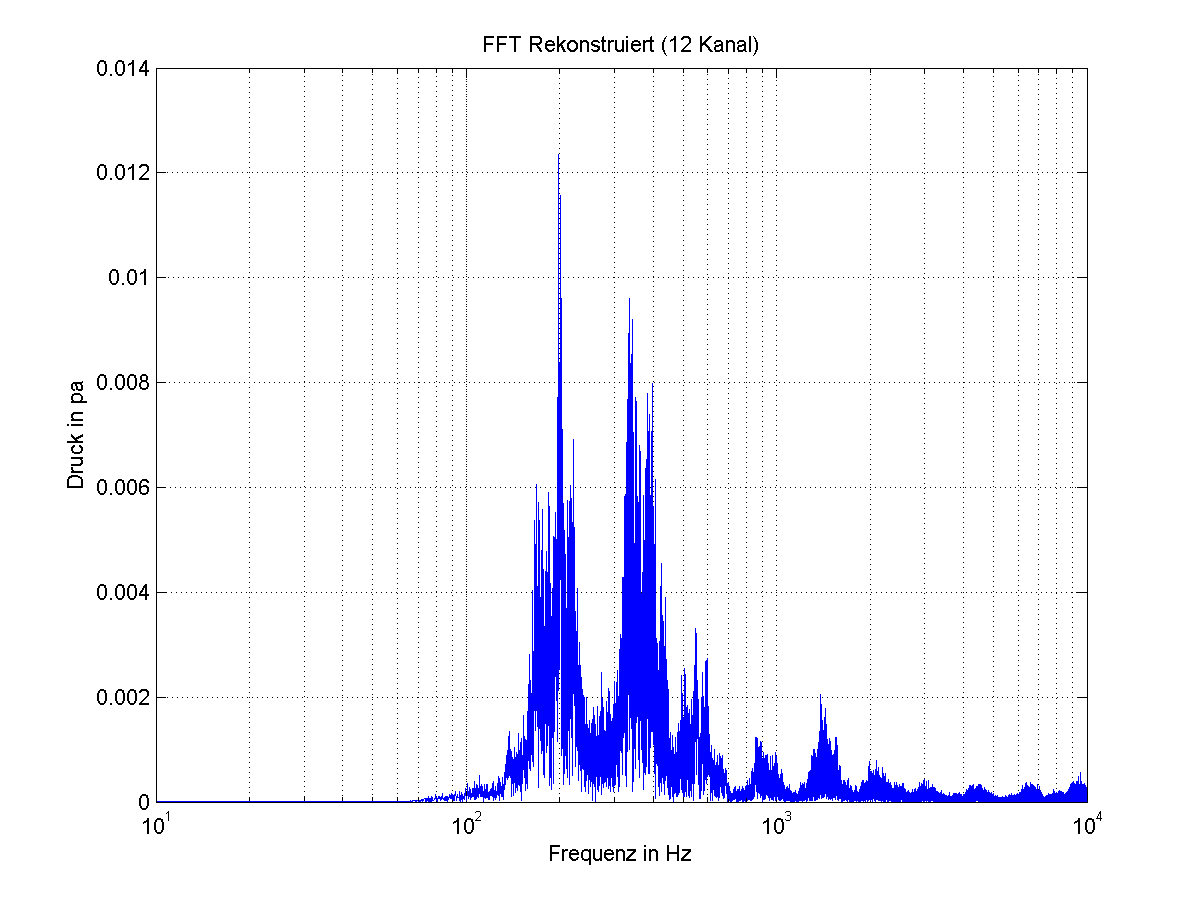
\includegraphics[width=0.5\textwidth]{img/fft_rec_12.png}
	\caption{Langzeitspektrum rekonstruiert von 12 Kanälen}
	\label{fig:fft-rec-12}
\end{figure}




\end{document}


